\documentclass[12pt, a4paper, oneside]{book}
\usepackage[spanish]{babel}
\usepackage[utf8]{inputenc}
%%%%%%%%%%%%%%%%%%%%%%%%%%%%%%%%%%
%
% AQUI SE TIENE LO NECESARIO Y MÁS
% 
% Ambientes de cuadros
% Dibujar Funciones
% Dibujar Tableros
% Creación de código fuente
% estilos, tamaños, cabeceras y pie de página
%
%%%%%%%%%%%%%%%%%%%%%%%%%%%%%%%%%%%
%
% Aqui se incluyen un conjunto de instrucciones y paquetes
% necesarios para todo lo que se quiera escribir
% NOTA: es evidente que el creador de la plantilla NO HA ESCRITO
% NINGUN PAQUETE DE LOS DE ABAJO
%
% Ha recopilado y modificado todo lo que él considera necesario
%
%%%%%%%%%%%%%%%%%%%%%%%%%%%%%%%%%%%




\usepackage{xparse}
\usepackage{multirow}
\usepackage[margin=1in]{geometry} 
\usepackage{amsmath,amsthm,amssymb}
\usepackage{booktabs}
\usepackage{tikz}
\usepackage{mdframed}
\usepackage{emptypage}
\usepackage{esvect}
\usetikzlibrary{arrows,positioning,fit,shapes,calc}
\usepackage{framed}
\usepackage{fancyhdr} 
\usepackage[
    type={CC},
    modifier={by-nc},
    version={4.0},
]{doclicense}
\pagestyle{fancy} 
\usepackage{chessboard}
\storechessboardstyle{5x5}{maxfield=e5}

%%%%%%%%%%%%%%%%%%%%%%%%%%%%%%%%%%%%%%%%%%%%%%%%%%
%CAMBIAR X1 Z1 Y A1 para el documento de TFG
\lhead[GNU Octave]{}
\rhead[]{GNU Octave}
\renewcommand{\headrulewidth}{0.5pt}
\lfoot[OTEA - Curso]{David Pacios Izquierdo}
\renewcommand{\footrulewidth}{0.5pt}
%%%%%%%%%%%%%%%%%%%%%%%%%%%%%%%%%%%%%%%%%%%%%%%%%%

\usetikzlibrary{calc,angles,positioning,intersections,quotes,decorations.markings}
\usepackage{tkz-euclide}
\usetkzobj{all}
\usepackage{pgfplots}
\usepackage{graphicx}
\usepackage{subfigure}
\usepackage{float}
\usepackage{listings}
\usepackage{xcolor}
\usepackage{multicol}
\pgfplotsset{compat=1.5}

%%%%%%%%%%%%%%%%%%%%% Dibujar funciones 
% https://es.sharelatex.com/learn/Pgfplots_package
% http://pgfplots.sourceforge.net/gallery.html
%%%%%%%%%%%%%%%%%%%%% Oficial documentation
% http://pgfplots.sourceforge.net/pgfplots.pdf
% http://pgfplots.sourceforge.net/pgfplotstable.pdf
%%%%%%%%%%%%%%%%%%%%%%%%%%%%%%%%%%%%%%%%%%%%%%%%%%%%%%%%%%%%%%%%%
\newcommand{\N}{\mathbb{N}}
\newcommand{\Z}{\mathbb{Z}}
\newcommand{\R}{\mathbb{R}}
\newcommand{\Q}{\mathbb{Q}}
\newcommand{\fd}{\rightarrow}
\newcommand{\cont}{\subset}
%%%%%%%%%%%%%%%%%%%%%%%%%%%%%%%%%%%%%%%%%%%%%%%%%%%%%%%%%%%%%%%%%
\lstset { %
    language=C++,
    backgroundcolor=\color{black!5}, % set backgroundcolor
    basicstyle=\footnotesize,% basic font setting
}
\lstset { %
    language=Octave,
    backgroundcolor=\color{black!5}, % set backgroundcolor
    basicstyle=\footnotesize,% basic font setting
}
\newenvironment{theorem}[2][Teorema]{\begin{framed}\begin{trivlist}
\item[\hskip \labelsep {\bfseries #1}\hskip \labelsep {\bfseries #2.}]}{\end{trivlist}\end{framed}}
\newenvironment{regla}[2][Regla]{\begin{trivlist}
\item[\hskip \labelsep {\bfseries #1}\hskip \labelsep {\bfseries #2.}]}{\end{trivlist}}
\newenvironment{axioma}[2][Axioma]{\begin{trivlist}
\item[\hskip \labelsep {\bfseries #1}\hskip \labelsep {\bfseries #2.}]}{\end{trivlist}}
\newenvironment{lemma}[2][Lemma]{\begin{trivlist}
\item[\hskip \labelsep {\bfseries #1}\hskip \labelsep {\bfseries #2.}]}{\end{trivlist}}
\newenvironment{exercise}[2][Ejercicio]{\begin{trivlist}
\item[\hskip \labelsep {\bfseries #1}\hskip \labelsep {\bfseries #2.}]}{\end{trivlist}}
\newenvironment{reflection}[2][Reflection]{\begin{trivlist}
\item[\hskip \labelsep {\bfseries #1}\hskip \labelsep {\bfseries #2.}]}{\end{trivlist}}
\newenvironment{proposition}[2][Proposicion]{\begin{trivlist}
\item[\hskip \labelsep {\bfseries #1}\hskip \labelsep {\bfseries #2.}]}{\end{trivlist}}
\newenvironment{corollary}[2][Corolario]{\begin{trivlist}
\item[\hskip \labelsep {\bfseries #1}\hskip \labelsep {\bfseries #2.}]}{\end{trivlist}}

\pgfplotsset{soldot/.style={color=blue,only marks,mark=*}} \pgfplotsset{holdot/.style={color=blue,fill=white,only marks,mark=*}}

\ExplSyntaxOn
\NewDocumentCommand{\ruffini}{mmmm}
 {% #1 = polynomial, #2 = divisor, #3 = middle row, #4 = result
  \franklin_ruffini:nnnn { #1 } { #2 } { #3 } { #4 }
 }

\seq_new:N \l_franklin_temp_seq
\tl_new:N \l_franklin_scheme_tl
\int_new:N \l_franklin_degree_int

\cs_new_protected:Npn \franklin_ruffini:nnnn #1 #2 #3 #4
 {
  % Start the first row
  \tl_set:Nn \l_franklin_scheme_tl { #2 & }
  % Split the list of coefficients
  \seq_set_split:Nnn \l_franklin_temp_seq { , } { #1 }
  % Remember the number of columns
  \int_set:Nn \l_franklin_degree_int { \seq_count:N \l_franklin_temp_seq }
  % Fill the first row
  \tl_put_right:Nx \l_franklin_scheme_tl
   { \seq_use:Nnnn \l_franklin_temp_seq { & } { & } { & } }
  % End the first row and leave two empty places in the next
  \tl_put_right:Nn \l_franklin_scheme_tl { \\ & & }
  % Split the list of coefficients and fill the second row
  \seq_set_split:Nnn \l_franklin_temp_seq { , } { #3 }
  \tl_put_right:Nx \l_franklin_scheme_tl
   { \seq_use:Nnnn \l_franklin_temp_seq { & } { & } { & } }
  % End the second row
  \tl_put_right:Nn \l_franklin_scheme_tl { \\ }
  % Compute the \cline command
  \tl_put_right:Nx \l_franklin_scheme_tl
   {
    \exp_not:N \cline { 2-\int_to_arabic:n { \l_franklin_degree_int + 1 } }
   }
  % Leave an empty place in the third row (no rule either)
  \tl_put_right:Nn \l_franklin_scheme_tl { \multicolumn{1}{r}{} & }
  % Split and fill the third row
  \seq_set_split:Nnn \l_franklin_temp_seq { , } { #4 }
  \tl_put_right:Nx \l_franklin_scheme_tl
   { \seq_use:Nnnn \l_franklin_temp_seq { & } { & } { & } }
  % Start the array (with \use:x because the array package
  % doesn't expand the argument)
  \use:x
   {
    \exp_not:n { \begin{array} } { r | *{\int_use:N \l_franklin_degree_int} { r } }
   }
  % Body of the array and finish
  \tl_use:N \l_franklin_scheme_tl
  \end{array}
 }
\ExplSyntaxOff
\usepackage{mdframed}
\newdimen\arrowsize
\pgfarrowsdeclare{squarea}{squarea}
{
  \arrowsize=0.4pt
  \advance\arrowsize by.275\pgflinewidth%
  \pgfarrowsleftextend{+-\arrowsize}
  \advance\arrowsize by.5\pgflinewidth
  \pgfarrowsrightextend{+\arrowsize}
}
{
  \arrowsize=0.4pt
  \advance\arrowsize by.275\pgflinewidth%
  \pgfsetdash{}{+0pt}
  \pgfsetroundjoin
  \pgfpathmoveto{\pgfqpoint{1\arrowsize}{4\arrowsize}}
  \pgfpathlineto{\pgfqpoint{-7\arrowsize}{4\arrowsize}}
  \pgfpathlineto{\pgfqpoint{-7\arrowsize}{-4\arrowsize}}
  \pgfpathlineto{\pgfqpoint{1\arrowsize}{-4\arrowsize}}
  \pgfpathclose
  \pgfusepathqfillstroke
}

\pgfarrowsdeclare{open squarea}{open squarea}%{{-.5bp}{8.5bp}}
{
  \arrowsize=0.4pt
  \advance\arrowsize by.275\pgflinewidth%
  \pgfarrowsleftextend{+-.5\pgflinewidth}
  \advance\arrowsize by7\arrowsize
  \advance\arrowsize by.5\pgflinewidth
  \pgfarrowsrightextend{+\arrowsize}
}
{
  \arrowsize=0.4pt
  \advance\arrowsize by.275\pgflinewidth%
  \pgfsetdash{}{+0pt}
  \pgfsetroundjoin
  \pgfpathmoveto{\pgfqpoint{8\arrowsize}{4\arrowsize}}
  \pgfpathlineto{\pgfqpoint{0\arrowsize}{4\arrowsize}}
  \pgfpathlineto{\pgfqpoint{0\arrowsize}{-4\arrowsize}}
  \pgfpathlineto{\pgfqpoint{8\arrowsize}{-4\arrowsize}}
  \pgfpathclose
  \pgfusepathqstroke
}


\makeatletter
\newdimen\tempa
\newdimen\tempb
\pgfdeclareshape{diamond in circle}{
\inheritsavedanchors[from=diamond] 
\inheritsavedanchors[from=circle] 
\inheritanchorborder[from=circle]
\inheritanchor[from=circle]{center}
\inheritanchor[from=circle]{radius}
\inheritanchor[from=circle]{north}
\inheritanchor[from=circle]{south}
\inheritanchor[from=circle]{east}
\inheritanchor[from=circle]{west}
\inheritanchor[from=circle]{anchorborder}
  \saveddimen\radius{

    \pgf@ya=.5\ht\pgfnodeparttextbox%
    \advance\pgf@ya by.5\dp\pgfnodeparttextbox%
    \pgfmathsetlength\pgf@yb{\pgfkeysvalueof{/pgf/inner ysep}}%
    \advance\pgf@ya by\pgf@yb%

    \pgf@xa=.5\wd\pgfnodeparttextbox%
    \pgfmathsetlength\pgf@xb{\pgfkeysvalueof{/pgf/inner xsep}}%
    \advance\pgf@xa by\pgf@xb%

    \pgf@process{\pgfpointnormalised{\pgfqpoint{\pgf@xa}{\pgf@ya}}}%
    \ifdim\pgf@x>\pgf@y%
        \c@pgf@counta=\pgf@x%
        \ifnum\c@pgf@counta=0\relax%
        \else%
          \divide\c@pgf@counta by 255\relax%
          \pgf@xa=16\pgf@xa\relax%
          \divide\pgf@xa by\c@pgf@counta%
          \pgf@xa=16\pgf@xa\relax%
        \fi%
      \else%
        \c@pgf@counta=\pgf@y%
        \ifnum\c@pgf@counta=0\relax%
        \else%
          \divide\c@pgf@counta by 255\relax%
          \pgf@ya=16\pgf@ya\relax%
          \divide\pgf@ya by\c@pgf@counta%
          \pgf@xa=16\pgf@ya\relax%
        \fi%
    \fi%
    \pgf@x=\pgf@xa%

    \pgfmathsetlength{\pgf@xb}{\pgfkeysvalueof{/pgf/minimum width}}%
    \pgfmathsetlength{\pgf@yb}{\pgfkeysvalueof{/pgf/minimum height}}%
    \ifdim\pgf@x<.5\pgf@xb%
        \pgf@x=.5\pgf@xb%
    \fi%
    \ifdim\pgf@x<.5\pgf@yb%
        \pgf@x=.5\pgf@yb%
    \fi%

    \pgfmathsetlength{\pgf@xb}{\pgfkeysvalueof{/pgf/outer xsep}}%
    \pgfmathsetlength{\pgf@yb}{\pgfkeysvalueof{/pgf/outer ysep}}%
    \ifdim\pgf@xb<\pgf@yb%
      \advance\pgf@x by\pgf@yb%
    \else%
      \advance\pgf@x by\pgf@xb%
    \fi%
  }
\backgroundpath{
    \tempa=\radius
    \pgfmathsetlength{\pgf@xb}{\pgfkeysvalueof{/pgf/outer xsep}}%
    \pgfmathsetlength{\pgf@yb}{\pgfkeysvalueof{/pgf/outer ysep}}%
    \ifdim\pgf@xb<\pgf@yb%
      \advance\tempa by-\pgf@yb%
    \else%
      \advance\tempa by-\pgf@xb%
    \fi%
    \pgfpathmoveto{\centerpoint\advance\pgf@x by\radius}%
    \pgfpathlineto{\centerpoint\advance\pgf@y by\radius}%
    \pgfpathlineto{\centerpoint\advance\pgf@x by-\radius}%
    \pgfpathlineto{\centerpoint\advance\pgf@y by-\radius}%
    \pgfpathclose%
  }
\behindbackgroundpath{
    \tempa=\radius%
    \pgfmathsetlength{\pgf@xb}{\pgfkeysvalueof{/pgf/outer xsep}}%
    \pgfmathsetlength{\pgf@yb}{\pgfkeysvalueof{/pgf/outer ysep}}%
    \ifdim\pgf@xb<\pgf@yb%
      \advance\tempa by-\pgf@yb%
    \else%
      \advance\tempa by-\pgf@xb%
    \fi%
    \pgfpathcircle{\centerpoint}{\tempa}%
  }
}
\makeatother

\newcommand{\parameter}[1]{$\langle\mbox{#1}\rangle$}
\usepackage{enumitem}
\setlength{\parindent}{12pt}
\renewcommand{\theenumi}{\Alph{enumi}}

\newcommand{\pascal}{\LARGE${\displaystyle \mathbf {P\!\!^{{}_{\scriptstyle A}}\!\!\!\!\!\;\;S\!_{\displaystyle C}\!A\!\!^{{}_{\scriptstyle L}}}}$}

\newcommand{\teflon}{\LARGE${\displaystyle \mathbf {T\!^{{}_{\scriptstyle E}}\!\!\!\!\;\;F\!_{\displaystyle L}\!O\!^{{}_{\scriptstyle N}}}}$}
%%%%%%%%%%%%%%%%%%%%%%%%%%%%%%%%%%%%%%% Más creaciones de Pascal



%%%%%%%%%%%%%%%%%%%%%%%%%%%
%
%      TeFloN V 1.2
%
%   Plantilla para TFGs
%
%   by Blai3e Pascal 
%    (David Pacios)
%
%%%%%%%%%%%%%%%%%%%%%%%%%%%

\begin{document}
\pagenumbering{Roman}
%%%%%%%%%%%%%%%%%%%%%%%%%%%%%%%%%%%%%%%%%%%%
%        TeFloN 1.0
%
% Plantilla para TFGs básica:
%
% title.tex dentro de la carpeta data
% Este documento incluye todo lo necesario de la plantilla
% Se basa en TeXiS de una forma más básica para usar en TFGs
% 
% Los datos modificables están marcados
%
%%%%%%%%%%%%%%%%%%%%%%%%%%%%%%%%%%%%%%%%%%%%




\thispagestyle{empty}
\vspace*{9mm}
\begin{center}
    \rule[0.5ex]{\linewidth}{2pt}\vspace*{-\baselineskip}\vspace*{3.2pt}\\
    \rule[0.5ex]{\linewidth}{2pt}\\
    
    {\textbf{Análisis de perspectivas de género en películas Disney} }\\[4mm] %Titulo del TFG
    {\Large \textit{Versión 0.1}}\\ %Subtitulo del TFG
    \rule[0.5ex]{\linewidth}{1pt}\vspace*{-\baselineskip}\vspace{3.2pt}
    \rule[0.5ex]{\linewidth}{2pt}\\
    \vspace{6.5mm}
    {\large Por}\\ 
    \vspace{6.5mm}
    {
        \large{\textsc{Alapont Tomás Pablo}},
        \large{\textsc{García Couto Carmen}},
        \large{\textsc{Jimenez Garrido Marina}},
        \large{\textsc{del Pino Castilla Victor}}\&
        \large{\textsc{Ruiz Casanova Leila}}
    }\\ %Nombres de los autores
    \vspace{11mm}
    
\includegraphics[scale=0.3]{Images/logo_UCM.jpg}\\ %Logo de la UCM
    \vspace{6mm}
    {\large \textsc{Ética Legislación y Profesión}\\  %Departamento del profesor que es el tutor
    \textsc{Facultad de Informática}}\\ %Facultad para la que se hace
    \vspace{11mm}
    \begin{minipage}{12cm}
    Un breve análisis de las perspectivas de género en películas Disney a lo largo del tiempo
    %Cuadro de presentación del TFG
    \end{minipage}\\
    \vspace{9mm}
    {\large\textsc{201812}} %Fecha de finalización o presentación
    \vspace{12mm}
\end{center}

%\newpage
\thispagestyle{empty}
\begin{flushleft} © Copyright (Alapont Tomás Pablo, del Pino Castilla Víctor, García Couto Carmen, Jiménez Garrido Marina, Ruiz Casanova Leila)

Todo esto esta bajo los derechos de autor. 
\vspace{16mm}

\begin{tabular}{@{}lp{\textwidth-10em}}
Año: Fecha  \\
Titulo: Titulo de la obra\\
Autor: Autor o autores\\
\end{tabular}
\end{flushleft} No es necesario pero se puede agregar, quedaría bien si se imprime en cuero por ejemplo porque estaría en la primera página útil, si no, queda raro.
\newpage
\chapter*{Sobre ASCII}
\noindent
\begin{multicols}{2}
\noindent
ASCII es la asociación a la que pertenezco (y de la que en el momento de la creación de este manual, presido) es una asociación creada en 1993 con la idea de reunir y tener un equilibrio entre el conocimiento y el ocio. Uno no excluye el otro, la idea de poder trabajar de forma distinta, como una familia, es la que se lleva intentando mostrar desde el comienzo.
\begin{figure}[H]
    \centering
    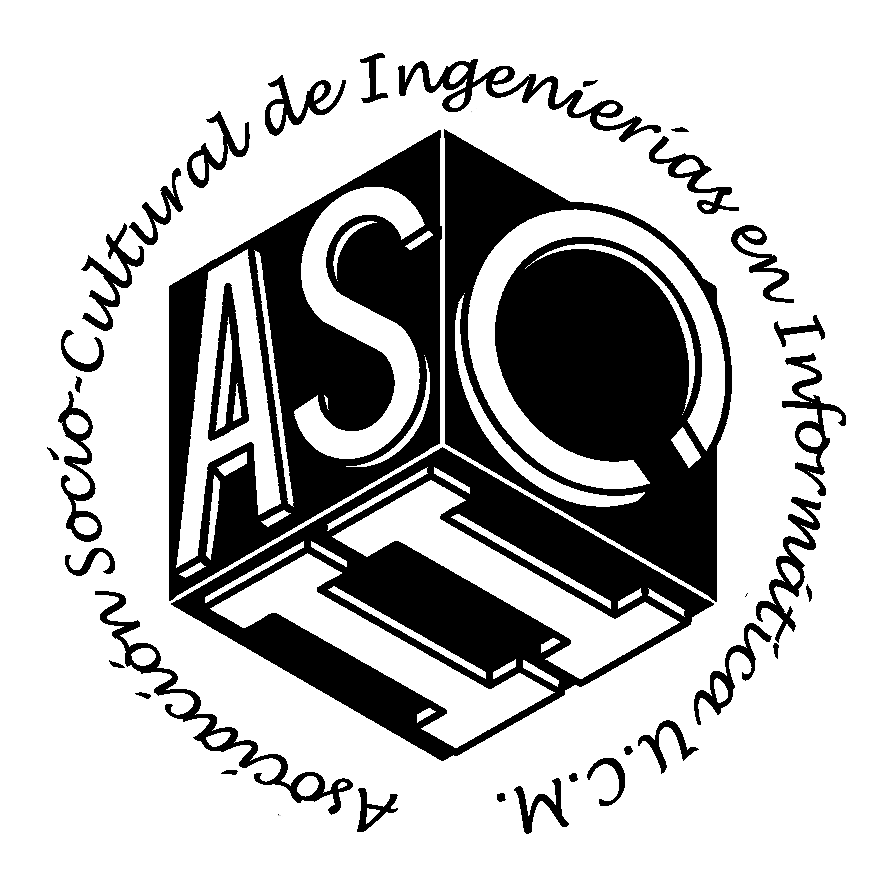
\includegraphics[width=5cm]{Images/logo_ASCII.png}
    \caption{\textit{Logo de la asociación ASCII}}
\end{figure}
\noindent
En los últimos años hemos tenido el honor de poder participar en iniciativas interesantes como:
\begin{itemize}
    \item \textbf{FDIst} (Grupo de seguridad de la Facultad de Informática)
    \item \textbf{OTEA} (Oficina de Software Libre de la UCM)
    \item \textbf{GamersParty} (Colaboración con LAG: Asociación de videojuegos de la UCM) con motivo solidario.
    \item \textbf{Cryptoparty:} Evento de ciberseguridad.
    \item \textbf{Cursos, talleres y Clases de apoyo.}
\end{itemize}
\noindent
Mantenemos una gran relación con el decanato, gerencia y personal docente de la Facultad de Informática. También mantenemos una gran relación con otras facultades gracias a la iniciativa de \textbf{``El Concilio de asociaciones''}. Podemos contar con orgullo como muchos de nuestros socios han acabado investigando o siendo profesores de la misma facultad. Actualmente seguimos teniendo esa mentalidad de ayudar a todos los alumnos con nuestros talleres, conferencias, cursos y de seguir mostrando ese ambiente de ocio friky que tanto nos caracteriza. Entre estas actividades destacamos:
\begin{itemize}
    \item \textbf{Sesiones de ROL} con masters expertos.
    \item \textbf{Préstamo de juegos de mesa} para uso y disfrute de todos.
    \item \textbf{Comidas y celebraciones} (Navidad, Halloween) con eventos temáticos.
    \item Concurso de comer Gofres y Chocolate.
\end{itemize}
\noindent
En el año 2018 también inauguramos, gracias a gerencia de la facultad de informática, al Ayuntamiento de Madrid, a cuidado de jardines de la UCM y a un error del presidente, \textbf{un estupendo bosque con 3 árboles} propiedad de la asociación.
\end{multicols}

\vfill
Más información: \url{https://ascii.fdi.ucm.es/}
\newpage
\chapter*{Sobre \teflon}
\noindent
\textsc{Teflon(cc0 1.0(documentación) MIT(código))%\cite{dPaciosTeflon}% 
es una plantilla de \LaTeX\phantom{} creada por David Pacios Izquierdo con fecha de Enero de 2018. Con atribuciones de uso CC0.}\\\\
\noindent
Esta plantilla fue desarrollada para facilitar la creación de documentación profesional para Trabajos de Fin de Grado o Trabajos de Fin de Máster. La versión usada es la 1.3.\\\\
\noindent
V:\textsc{1.3 Overleaf V2 with pdfLaTeX, margin 1in, Oneside}
\vfill
\noindent
\textsc{\textbf{\underline{Contacto}}\\ \textbf{Autor:} David Pacios Izquiero \\ \textbf{Correo:} \url{dpacios@ucm.es}\\ \textbf{ASCII:} \url{asciifdi@gmail.com}\\ Despacho 110 - Facultad de Informática}

\addtocontents{toc}{\hfill \textbf{Página} \par}
\tableofcontents
%%%% Chapters
\noindent %Agregar siempre que de por culo la indentación
\chapter{Estado del arte}
\noindent
%Que hay hecho sobre el tema

%Aquí es donde mola meter referencias bibliográficas, se pueden sacar desde google scholar, pero con que me las dejéis anotadas con un comentario me vale. Y ya me encargaré yo de engancharla

Esto es un ejemplo de frase que está respaldada con una fuente \cite{england2011gender}.
Esta otra frase necesita una fuente que está en este libro %Alicia en el pais de las maravillas - Lewis Carroll%Estado del Arte
\noindent %Agregar siempre que de por culo la indentación
\chapter{Análisis del problema} 
\noindent
%Descripción concreta de qué vamos a resolver, como vamos a solucionar el hambre en el mundo y cómo nuestro trabajo essupone el fin de los problemas del hombre tal y como los conocemos

%Análisis del problema
\noindent %Agregar siempre que de por culo la indentación
\chapter{Solución}
%Si el anterior capítulo es la descripción del problema, este es la descripción de la solución, es decir, como vamos a obtener unos resultados y qué herramientas vamos a utilizar. Como vamos a aplicarlas y por qué son correctas.
    Nuestro primer planteamiento ha sido solucionar el problema de medir algo subjetivo. Ya que una película puede parecer que deja a las mujeres en un papel mas o menos sumiso. Pero no deja de ser subjetivo. Esto imposibilita el realizar una métrica razonable. Por ello, el primer trabajo que hemos realizado es la búsqueda de métricas. Mas adelante hemos sopesado estas métricas para poder puntuar cada película y así poder compararla.
\section{Datos a analizar}
    Dentro de las distintas métricas buscadas, hemos considerado las siguientes:
    \begin{itemize}
        \item \textbf{Test de Bechdel:} Valora si en una película la carga argumental pertenece exclusivamente a los varones o si las mujeres obtienen protagonismo. La valoración es booleana.
        \item \textbf{Sexo de los protagonistas:} Atendiendo únicamente a los protagonistas, se valora el balance entre un género u otro. Aquí hablamos de los personajes sobre los que versa la historia. Generalmente estos personajes se pintan como modelos a seguir, y el mensaje que se obtiene es el de que representan lo positivo y los valores a adoptar. Se obtiene una fracción $[-\infty,\infty]$
        \item \textbf{Sexo y número de los personajes secundarios:} Al igual que valoramos el sexo de los protagonistas, es importante valorar el sexo de los personajes que compartan la carga argumental sin protagonizar la historia. Esto otorga una idea sobre cómo está poblado el mundo. Se obtiene una fracción $[0,\infty]$
        \item \textbf{Sexo de los antagonistas:} Tan importante como los protagonistas, es considerar a los antagonistas. De la misma manera que unos plasman roles positivos, ideas a seguir, arquetipos que cumplir y costumbres a adoptar. Un antagonista es una visión de los valores contrarios. Una parte importante de la comunicación audiovisual es la de plasmar gráficamente cómo es un personaje. De esta manera asociamos tonos oscuros con intenciones malignas.
        \item \textbf{Tiempo en pantalla:} Seleccionando a los personajes con mas peso en la historia y separándolos por sexo, independientemente de si cumplen uno u otro arquetipo. Plasmamos su tiempo en pantalla como una correlación de cuanto puede afectar la presencia de un personaje a la valoración de la película. Se obtiene un ratio $[0,1]$
        \item \textbf{Cantidad de guión:} Consideramos que hay una correlación entre la cantidad de líneas que hay en un guión atribuidas a un personaje. Esto puede ser especialmente problemático con personajes que no se comunican verbalmente, o en los que quedan registradas líneas que puedan decir de fondo sin que sean parte principal de la película. Un ejemplo de esto puede ser Dumbo o Campanilla.
        \item \textbf{Definición de arcos argumentales}. Sabiendo que actualmente no se construyen historias partiendo de cero, sino que la tradición popular de contar historias emplea ciertos bloques constructivos para formar. Desde el empleo de ciertas motivaciones recurrentes en las historias, como la princesa en apuros. La plantilla de hacer histórias del monomito también llamado \textit{el mito de héroe} \cite{campbell1989hero}. O la que ha hecho a Disney famosa de reinterpretar obras de dominio público como Macbeth reinterpretada en el Rey león, Los cuentos de los hermanos Grimm, o las últimas reinterpretaciones de sus reinterpretaciones en la Bella y la Bestia.
    \end{itemize}
    
    Ninguna de estas métricas, por si mismas, soluciona el problema de medir objetivamente algo subjetivo. Y Consideramos que ninguna lo hará. Es por esto que consideramos todas las métricas a la vez y las ponderamos. Para ayudarnos de la ley de los grandes números \cite{LeyDeGrandesNumeros}, consideramos que las distintas métricas nos cuentan todas, lo alienada que se encuentra la película de carecer de sesgos hacia uno u otro lado. Así podemos ponerlas en común y compensar los fallos de una u otra con las demás métricas.
    
    Otro problema que ofrecen algunas métricas es la dificultad de implementarlas. En el caso del tiempo en pantalla. No hemos encontrado ninguna base de datos de películas en las que se ofrezcan estos datos. por lo tanto hemos tenido que realizarlo a mano para un subconjunto de las películas. Quedando para trabajos futuros la búsqueda o implementación de una herramienta que recopile estos datos o de una base de datos que los incorpore. Por esto, no hemos podido aplicar todas las métricas en todo el documento.


\section{Análisis manual}
    Ante la imposibilidad de analizar automáticamente el tiempo en pantalla hemos seleccionado diez películas para las que hemos cronometrado el tiempo desde cuatro hasta nueve de los personajes mas significativos de la película. No quiere decir los protagonistas o en general el lado con el que se identifica el espectador. Nos interesan los personajes que mas pueden aportar a la trama, se identifiquen con el espectador o en contra o simplemente ejerzan una influencia en la historia.
\section{Análisis automático}
Para realizar el análisis automático de los guiones se ha planteado una arquitectura de flujo ya que las operaciones a realizar son comunes y consecutivas a todos los guiones. Para esto se ha utilizado tecnología Python, desarrollada a medida para el proyecto. Todo el proyecto está alojado en el repositorio Disney.
Debido a la forma de flujos de pasos se procede a explicar estos de forma secuencial:
\begin{itemize}
    \item \textbf{Extracción de las líneas de guión} \\\\
        \textit{(Scripts: TreatMovies0X.py, TreatMovies1X.py, TreatMovies2X.py)} En estos scripts se realiza la operación principal de obtención de información, extrayendo el nombre del personaje y las frases que aparecen en el guión, eliminado la información adicional que no es objeto de este análisis, como comentarios de movimiento de personajes y marcas de escenas. Debido a los diferentes formatos encontrados, los guiones se han catalogado en 23 tipos distintos, realizando el análisis línea a línea de cada uno de los ficheros disponibles.
    \item \textbf{Limpieza} \\\\
        \textit{(Scripts: TreatMovies3X.py)} En esta sección se limpian los textos obtenidos de caracteres y comentarios que si bien aparecen dentro de las entradas de cada uno de los personajes en el guión de la película, no son frases pronunciadas por los personajes y no deben tenerse en cuenta en el análisis.
    \item \textbf{Contar palabras}\\\\
        \textit{(Scripts: TreatMovies4X.py)} Una vez que tenemos limpios los textos de cada personaje, realizamos un conteo del número de palabras que aparecen en el guión de cada película, para cada uno de los personajes
    \item \textbf{Contabilizar por género}\\\\
        \textit{(Scripts: TreatMovies5X.py, TreatMovies6X.py, TreatMovies7X.py, TreatMovies8X.py, TreatMovies9X.py, TreatMovies10X.py)} Con la información obtenida, cuantas palabras tiene cada uno de los personajes, se realiza un análisis película a película obteniendo la suma total palabras pronunciadas diferenciadas por géneros.
    \item \textbf{Resultados finales}\\\\
        \textit{(Scripts: TreatMovies12X.py)} Por último se recorren todos los datos generados en el paso anterior y se genera un documento con el porcentaje de palabras pronunciadas por personajes femeninos
\end{itemize}%Solución
\noindent %Agregar siempre que de por culo la indentación
\chapter{Resultados}
%Descripción de los datos obtenidos. No es un análisis de la conclusión, llegará en el capitulo que viene. Es simplemente una ordenación de los datos
\section{Análisis automático}
    A partir del análisis automático descritos en el apartado anterior. Hemos obtenido una proporción entre el dialogo de varones y mujeres. Siendo 0\% exclusivo de los varones y 100\% exclusivo de las mujeres.
    
    \begin{figure}
        \centering
        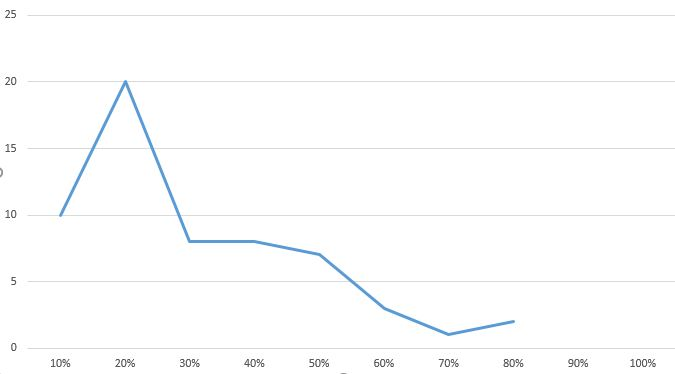
\includegraphics[scale=0.7]{Images/distribucion.jpg}
        \caption{ocurrencias en tramos del 10\% de proporción de diálogo por género}
    \end{figure}
    
\newpage
\section{Análisis manual}
    A partir del análisis manual hemos realizado preguntas diferentes, debido a la diferencia de las pruebas que hemos podido automatizar y las que no. Nuestra intención ha sido la de automatizar lo mas posible para poder abarcar el total de las películas de Disney y eventualmente poder mejorar la calidad de los datos. Pero nos hemos encontrado con diferentes fuentes y formatos para los mismos datos de cada película. Especialmente debido a la naturaleza intelectual de los datos y en menor medida debido a la falta de interés de normalizar estos parámetros. En el siguiente gráfico vemos una serie de películas ordenadas temporalmente con la tasa de tiempo de hombres y mujeres sin apreciarse especial inclinación a un lado u otro. Igualmente, en la suma total de tiempos se ve una desviación de la mitad, fácilmente atribuible al ruido.
    \begin{figure}
        \centering
        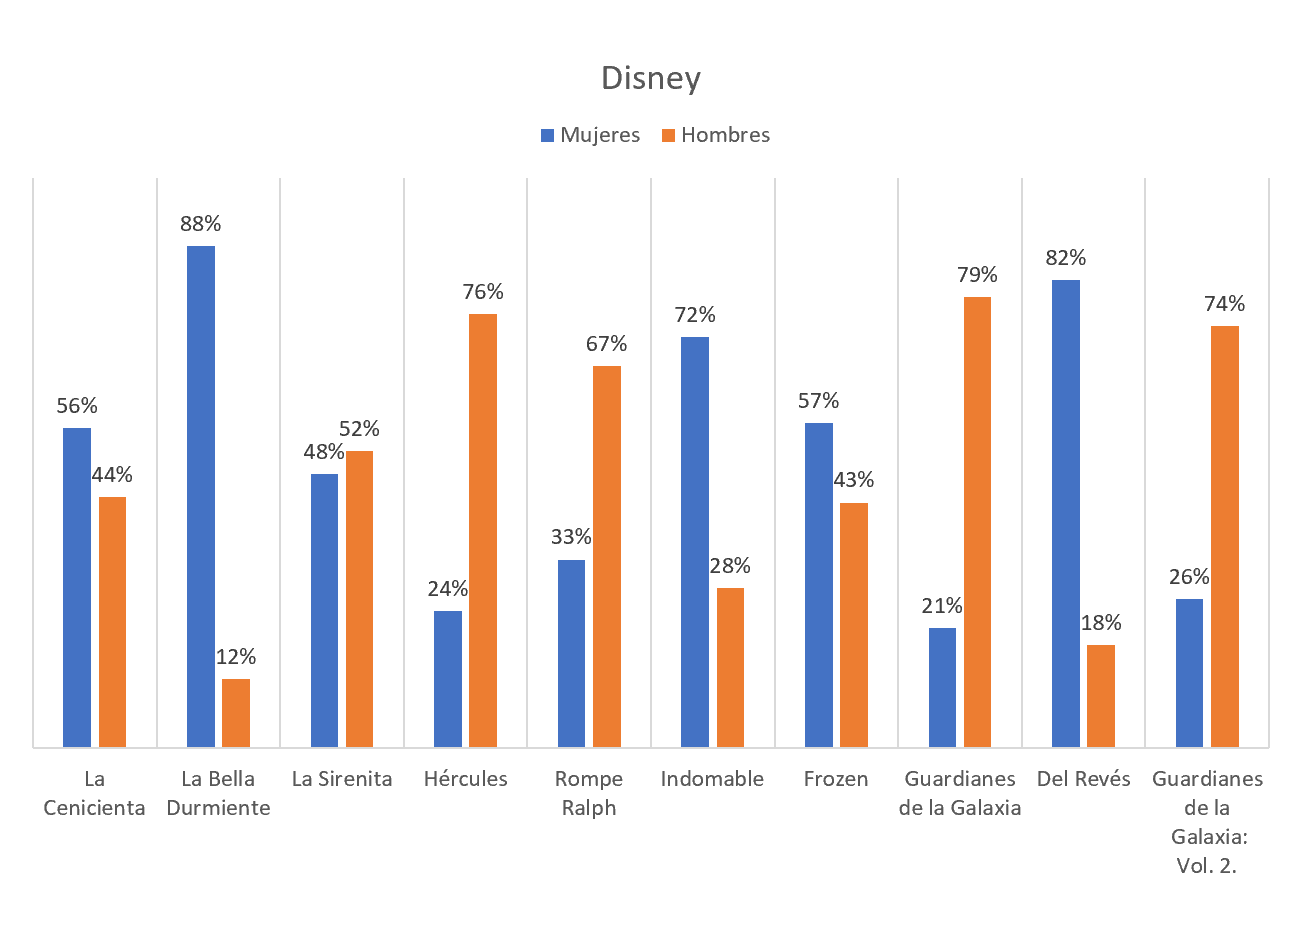
\includegraphics[scale=0.7]{Images/peliculas.png}
        \caption{Distribución de las líneas de diálogo por sexos y películas ordenadas por fecha de estreno}
    \end{figure}
    \begin{figure}
        \centering
        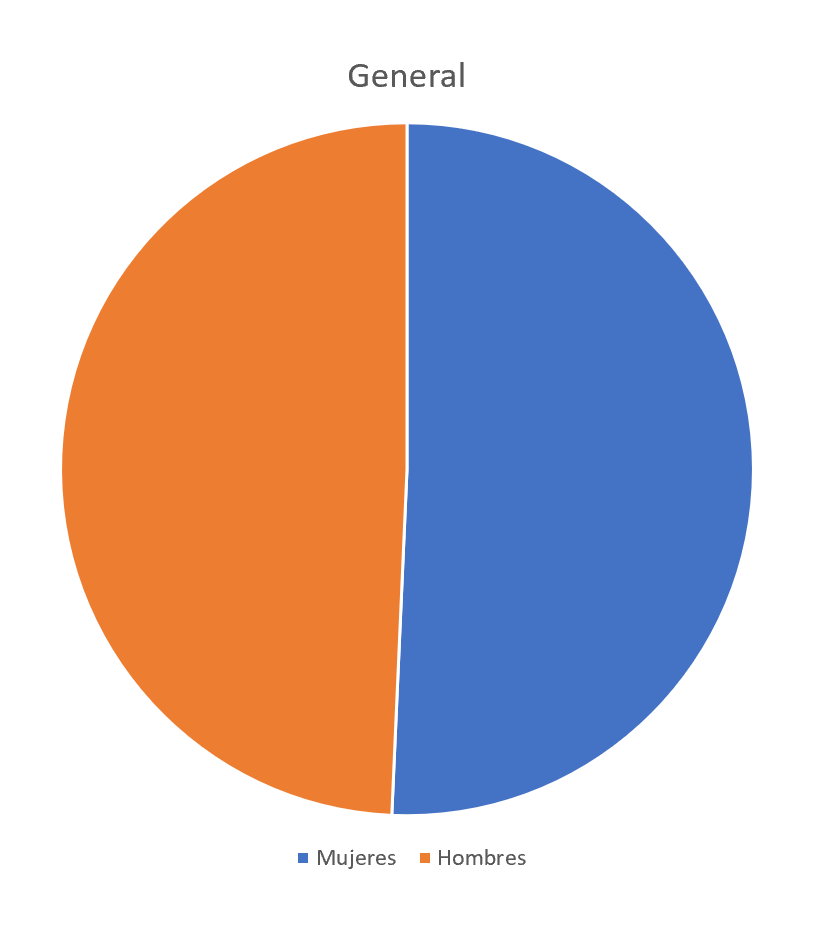
\includegraphics[scale=0.7]{Images/general.png}
        \caption{Distribución de las líneas de diálogo por sexos dentro de las películas analizadas}
    \end{figure}%Resultados
\noindent %Agregar siempre que de por culo la indentación
\chapter{Conclusiones}
% Una vez aplicado nuestro trabajo, que conclusiones hemos obtenido. Siempre de la manera mas objetiva posible, esto es, lo menos subjetivo posible
%Lo he copiado de la wiki
    Por todos los motivos expuestos consideramos que Disney muestra un rango de personajes lo suficientemente amplio como para decir que no existe un sesgo de género significativo, si no que hacen uso de los arquetipos necesarios para contar la historia en la que se centran en el momento. Historias que pueden estar basadas en a tradición oral o ser originales. Con una inversión del género de los personajes los argumentos no sufrirían ninguna alteración y no se incurriría en la percepción del sesgo de Género.
    
\section{Análisis de los datos automáticos}
    Ateniendonos a los datos recopilados automáticamente. Podemos ver una media del 25\%. Bastante descentrada de un 50\% que a priori sería lo ideal. Además hay una gran concentración entorno al 15\%. Un valor muy sesgado, especialmente considerando que incluye películas muy nuevas como Wall-e e Iron man, incluso con películas con multitud de protagonistas como la serie de los vengadores o Capitán America Civil war, donde uno podría esperar que el hecho de que el protagonista hable mucho mas que otros personajes, queda diluida en muchos mas personajes que podrían haber ofrecido mucha mas diversidad.
    
\section{Análisis de los datos manuales}
    El análisis manual \textit{(medición de tiempos)} muestra una dispersión de los datos demasiado grande comparado con una media bastante centrada. Esto es síntoma de poca correlación entre la diferencia de asignación de tiempo en pantalla por sexos o por tiempos. Es decir, No podemos asegurar fiablemente que si una película es mas vieja o mas nueva, vaya a implicar necesariamente que varones aparezcan mas o menos tiempo que mujeres.
    Por otro lado todas las historias comprobadas excepto una (\textit{Hércules}) pasan el test de Bechdel. Lo cual hace de esa única ocurrencia algo poco significativo.
    Con estos datos, podemos pensar que Disney genera unas historias poco sexualizadas o en las que el género importa poco.
    Como anécdota, el varón que mas tiempo permanece en pantalla es Rompe Ralph (59 minutos) y la mujer que mas tiempo aparece es Anna de Frozen (62 miutos). Ambos con tiempos similares.
    Brave es la película que hemos tratado que mas tiempo otorga a mujeres, ya que es principalmente la historia de una madre y su hija en un entorno bastante aislado. Los varones que aparecen lo hacen como un gag cómico mas que como elementos de la historia. Ocasionalmente como lo que Hitchcok denomina un McGuffin.
\section{Posible explicación de las discrepancias entre los diferentes datos}
    Los datos del análisis manual están hechos sobre pocas películas, mientras que el análisis automático se realiza sobre un pool mas grande. Aunque no es motivo suficiente para invalidar nungún conjunto de datos, si que merece un poco de prudencia y un análisis posterior. Que hemos detallado en el Trabajo futuro.%Conclusiones
\noindent %Agregar siempre que de por culo la indentación
\chapter{Trabajo futuro}
%A pesar de que acabamos de salvar a la humanidad y estamos camino de recoger el Nobel, es posible que nos hayamos dejado cosas por el camino, y quien mejor que nosotros para saber cómo se debe avanzar
A la hora de puntuar las películas nos hemos encontrado con diferentes obstáculos. Por un lado las métricas no son objetivas, y por lo tanto propensas a error. Por otro lado, algunas métricas utilizadas si son objetivas, pero no son representativas del sesgo de la película. El tiempo en pantalla no implica que una película sea mas o menos inclusiva, aunque puede haber una correlación. De esta manera, un trabajo futuro es la incorporación de nuevas métricas que permitan, gracias a la ley de los grandes números, converger hacia puntuaciones mas fiables de cada película.

Otro trabajo es, para las métricas que ya estamos midiendo, medirlas de forma mas precisa. Ya que una medición automática puede agilizar la incorporación de películas a la base de datos. Especialmente con algoritmos de reconocimiento de personajes basados en redes neuronales como los aplicados por programas de bancos de fotos, similares a los que pueden usar Facebook o Google.

Un estudio alternativo es el de considerar las diferentes métricas por separado independientemente de las demás y en conjunto a través de las diferentes películas. Pudiendo resultar en diferentes estudios en función del protagonismo de los personajes como la cantidad de antagonistas de cada sexo a lo largo de la historia.

Al igual que se puede mejorar la calidad de las métricas como ya hemos comentado en los dos puntos anteriores. Es importante también contar con una cantidad de muestras mayor. A la hora de escribir este trabajo Disney cuenta con 338 películas \cite{listaDisney}. Una lista que no incluye otras productoras asociadas y que también forman parte de la cultura popular. Incorporar cuantas mas películas fomenta una imagen mas clara de la evolución de las perspectivas de género en la cultura y el imaginario popular.

Otra parte que no medimos y que sería interesante llegar a medir es lo sexista del lenguaje. Ésto plantea sus propios problemas, especialmente por los parámetros a medir y como se miden y su contexto temporal.

Adicionalmente, a parte de incluir cuantas mas películas mejor, es importante sopesarlas según su impacto en la sociedad. Para lo cual habría que incluir nuevas métricas que capturar y medir. Ya que se debería sopesar su alcance, su visionado y tiempo desde la publicación (o reedición), para poder empezar a ver cuanto influye una u otra película en la sociedad de un momento dado. De esta manera conseguiríamos, no solo relacionar unas películas con otras, sino relacionar unas sociedades en el tiempo con otras. Lo cual implica enfrentarse con el problema de modelar cuanto afecta una película a la sociedad a lo largo del tiempo, lo cual no es un problema trivial. 
%Trabajos futuros
\newpage
\bibliographystyle{unsrt}
\bibliography{biblio}
\addcontentsline{toc}{chapter}{\protect\numberline{7}Bibliografía y enlaces de referencia}%0
\thispagestyle{empty}


%%%%%%%%%%%%%%%%%%%%%% COMENTAR ESTAS DOS LÍNEAS PARA QUITAR AUTORÍA
\vspace*{\fill} %
\doclicenseThis%
%%%%%%%%%%%%%%%%%%%%%%
\end{document}